\section{Overview}
\label{sec:overview}

\begin{figure*}
	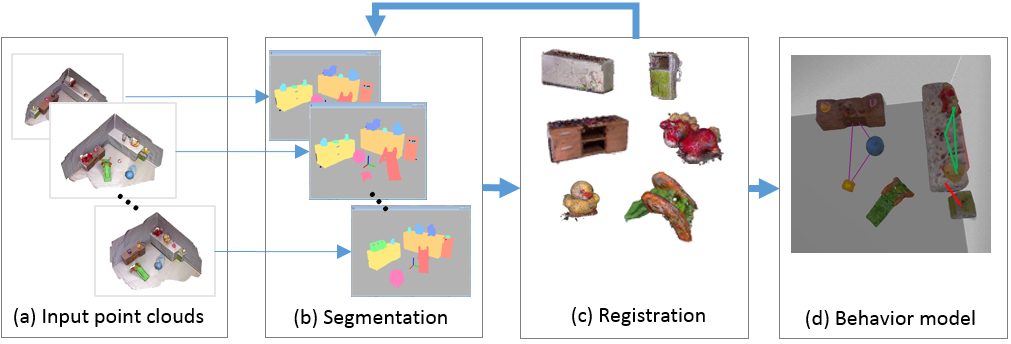
\includegraphics[width=1.0\textwidth]{figures/overview}
	\caption{System overview.}
	\label{fig:overview}
\end{figure*}

The objective of our algorithm is to recover object behaviors from a set of point clouds scanned at different times for an indoor scene.
%
To achieve this goal, objects and correspondences between objects and point clouds must be extracted. 
%
More specifically, our problem is to transfer the noisy and incomplete point-level data into object-level models and correspondences to understand the object behaviors in the scene.
%


Our system consists of two main steps, \emph{point cloud segmentation} and \emph{object registration}, as Figure~\ref{fig:overview} shows. 
The \textbf{input} is a set of point clouds scanned using a RGBD camera (a). 
We scan each scene at different times \blueemph{during a month} using a Microsoft Kinect V1. A set of dense point clouds are generated using a real-time fusion system~\cite{NieBner:2013:VoxelHashing}. 
%
It is burdensome to scan every detailed structure in a cluttered indoor scene. As a result, each point cloud is incomplete and noisy due to object occlusions.



We first segment each frame simply using \blueemph{region growing} (b).
There are very likely many wrong boundaries in the generated patches.
Then we cluster all the patches from all frames into $k$ clusters using $k$means. 
%
\cite{Jia20153D} have demonstrated the power of features based on bounding box in the segmentation of indoor objects.
Therefore, we design the descriptor of each patch as the cascades of length, width and height of its bounding box, mean and standard deviation of the distance of each point to its bounding box, percentage of closest points to the faces of its bounding box.  
The feature dimension is then reduced using PCA. 
\xj{Currently, this step is manually done.} 



In each cluster, the patches are registered using a joint registration method~\cite{Evangelidis-ECCV-2014} to produce the object model of this cluster (c).
%
There are inevitably wrong registration due to wrong clustering. 
Therefore, we project the generated object models back into each frame using the estimated transformation. 
Re-segmentation is performed using the model consistency and neighborhood information in each frame, as described in Sec.~\ref{sec:segmentation}.
By iteratively register resegmented patches and re-segment frames, our system converges to a set of well-registered 3D object models and accurate correspondence between object model and all point clouds. 
%
Then we learn the behavior model (d) based the object correspondences from all input point clouds (Sec.~\ref{sec:behavior}), then apply the behavior model into many applications (Sec.~\ref{sec:applications}). 




\comment{
\begin{enumerate}
\item  \emph{Registration/Labeling:} Given a sequence of RGBD data captured in different times and views, we first register \emph{all the RGBD images} to segment objects and detect motions according to their low-rank characteristics using Robust PCA~\cite{candes2011robust}.
%
Given the assumption that there are typically static objects, such as wall, floor and so on, moving objects can be treated as sparse noise and the static backgrounds can be separated and completed as low-rank part by the robust PCA.
The point clouds are then divided into two categories: static objects and dynamic objects.
Combing the separated sparse part and the low-rank part, \emph{object segmentation} is performed by combing the motion, depth, and appearance features in the RGBD images. 

\comment{
\emph{Progressive Object Modeling} Static objects are reconstructed based on geometry primitives/model database. Dynamic objects are typically small size, connected with a large static object. They can be reconstructed by combing the point clouds captured under different views.
}
%\emph{Spatial Distribution:} After each round of registration and labeling of the input RGBD images, we can refine the spatial distribution map of each object. The map describes its position, poses and so on in the indoor environment. The interconnection between objects are then progressively refined.


\item \emph{Function Analysis/Behavior Map:}  
With the segmented regions, objects should be identified according to their appearance and geometry features among the entire image sets. 
We build a dynamic behavior map including all of the objects in the scene. Each node is an object/a part of an object. The edges in the graph describe the spatial relationship between objects/parts.
The object behavior can be explored from its surrounding objects in the dynamic structure graph. With a dynamic behavior map, the RGBD data is re-segmented and re-labeled to obtain semantical consistency of the scene.

\end{enumerate}
}
	

 







